%% ==============================================
%%           Design and Implementation
%% ==============================================
%% Author: Fabian Sorn
%% ==============================================


\chapter{Design and Implementation of a Benchmark Framework}
\label{ch:application}

In this chapter, the findings from the previous chapters will be combined
to design and implement a benchmarking framework, which allows the user to benchmark charting operations, he has defined himself. 




%% ==============================================
%%          Python Graph Libraries
%% ==============================================

\section{Python Graph Libraries}
\label{sec:application:libraries}

When benchmarking different Python Graph libraries, we will focus our attention on two contenders for the implementation, which .

\subsection{Matplotlib}
\label{sec:application:libraries:matplotlib}

Matplotlib is probably the standard library for 2D data visualization in Python. It offers publication quality visualization as well as an interactive environment. The project was initialized by John D. Hunter as an easy to use Python 2D plotting library, especially for users familiar with Data Visualization in Matlab.
\cite{Matplotlib, MatplotlibHistory}

Matplotlibs central item is the \inlinecode{Python}{matplotlib.figure.Figure}. The Figure itself does not yet display anything, neither a plot with axes nor data. A plot is reffered as an \inlinecode{Python}{matplotlib.axes.Axes}. A figure can have multiple Axes in it. For each dimension in the data space the Axes contains \inlinecode{Python}{matplotlib.axis.Axis} objects, which represents the minimum and maximum data limit for each dimension of the data. An Axes object can be personalised thourgh axis labels and a title. In Matplotlib terminology, Artists are everything which is visible in a Figure. This includes, Labels, Line and Bar Graphs, Axis Items and more. The last crucial component is the Canvas, which is not really a visual component in the plot, but the component responsible for rendering the image.

Matplotlib is built for many different use cases. While showing data in \gls{gui} applications is one of them, it can be used for other use cases, like generating plots as images for publications. This is achieved by Matplotlib supporting different Backends. A Backend is the system, which allows you to use Matplotlib in these different use cases. All available Backends can be devided in interactive and hardcopy ones. An example for a interactive backend is in our case PyQt5, but other Frameworks like Tkinter or PyGTK are supported. Non interactive backends are for creating image files in different file formats like PNG, SVG, PDF and more.
\cite{MatplotlibIntro, PythonDataVis}

Listing \ref{listing:application:matplotlib} shows the creation of a window containing a plot representing a sinus curve in different ways. For interaction, MatPlotLib offers a Toolbar, which lets you select between different interaction modes like panning and zooming. As a backend Matplotlib's Qt5 backend was used. The resulting window can be seen in Screenshot \ref{a:fig:matplotlib:window}.

\lstinputlisting[
    caption=Definition of a Window containing a plot created with Matplotlib,
    language=python, 
    label=listing:application:matplotlib,
    firstline=4,
    lastline=35
]{resources/code/matplotlib_demo.py}

\subsection{PyQtGraph}
\label{sec:application:libraries:pyqtgraph}

PyQtGraph is a pure python plotting library. While not offering as many features as other Python plotting libraries like Matplotlib, PyQtGraph promises to offer much better Plotting performance. PyQtGraph was initialized by Luke Campagnola and is focused on providing plotting functionalities for engineering and science applications. It provides simple plots containing line graphs, scatter plots, bar graphs and more, but also offers widgets for image and video displaying, Region of Interest widgets, 3D visualization and more. Since our benchmarking efforts will be tightly focusing on the collected use cases, we will restrict our usage of its features mainly on plots with different data visualization. PyQtGraph uses Qt's Graphics View for drawing, which is a Framework for fast visualization of a large number of custom 2D items. A big advantage it offers is its fast performance and the possibility for the user to interact and transform the scene through for example zooming or rotation. \cite{GraphicsView}

Since PyQtGraph is built on top of Qt features, integrating it into Qt applications is very simple. The central component for plotting is the \inlinecode{Python}{pyqtgraph.PlotWidget}. Since it is derived from \inlinecode{Python}{QtWidgets.QWidget}, it is very simple to add to a window. When adding the plot widget to a window, it comes with different components on the inside, as seen in \ref{a:fig:pyqtgraph:content}. The central one is the \inlinecode{Python}{pyqtgraph.PlotItem}, which is the actual plot. The widget itself is only a wrapper for easy integration into Qt Applications. The PlotItem contains different components of the plot, including a \inlinecode{Python}{pyqtgraph.ViewBox}, which is the area data is visualized in, a \inlinecode{Python}{pyqtgraph.AxisItem}, which is representing the View Range of the View Box and a Title. Items which are actually representing a dataset are added to the View Box. For this, PyQtGraph is offering different types of representations like a \inlinecode{Python}{pyqtgraph.PlotDataItem} for Scatter Plots and Line Graphs or \inlinecode{Python}{pyqtgraph.BarGraphItem} for representing data in a bar graph.

Listing \ref{listing:application:pyqtgraph} shows the creation of a window containing a plot representing a sinus curve in different ways. It displays the same data sets in the same style as the example from \ref{sec:application:libraries:matplotlib}. For the Line Graph and Scatter Plot we can use \inlinecode{Python}{pyqtgraph.PlotDataItem}. For the Bar Graph we create a \inlinecode{Python}{pyqtgraph.BarGraphItem}. Each item can then be added to the plot. The resulting window can be seen in \ref{a:fig:pyqtgraph:window}.
\cite{PyQtGraphDoc}

\lstinputlisting[
    caption=Definition of a window containing a plot created with PyQtGraph,
    language=python, 
    label=listing:application:pyqtgraph,
    firstline=2,
    lastline=25
]{resources/code/pyqtgraph_demo.py}

\subsubsection{Extensions for PyQtGraph from \gls{aps}}
\label{sec:application:libraries:accpyqtgraph}
PyQtGraph has already seen adaption in projects at \gls{cern}, which needed fast plotting performance. To provide a more convenient and faster development experience, \gls{aps} is providing a extended version of PyQtGraph mainly adapted for usage in Runtime Monitoring Applications. This extension offers first of all the additions of important features missing in PyQtGraph and as second a convenient live data plotting layer.

One feature which PyQtGraph is lacking, is the ability to plot two ore more datasets on different y-axes. This feature is especially useful, when you are viewing and comparing data sets, whose values are in vastly different ranges on the y-axis. One example where this feature was heavily missing, was the use case described in section \ref{sec:usecases:linac}. As seen in the screenshot \ref{fig:linac4sourcegui} the plot in the upper right corner contains two axes on the left and right side. The left one is showing a range from approximately minus 35 to 15, while the right one shows a range from minus 15000 to 35000. To keep the plot interactive, the different data sets are displayed on different areas, which are \inlinecode{Python}{pyqtgraph.ViewBox}. The shown view range is displayed by an \inlinecode{Python}{pyqtgraph.AxisItem}. In the extension a layer describes one of these viewboxes together with its axis. Schema \ref{fig:application:pyqtgraph:layers} show how mulitple layers are stacked on top of each other to build a single plot. The big advantage is, that each layer can be moved individually by the user of the application.

\begin{figure}[h]
    \centering
    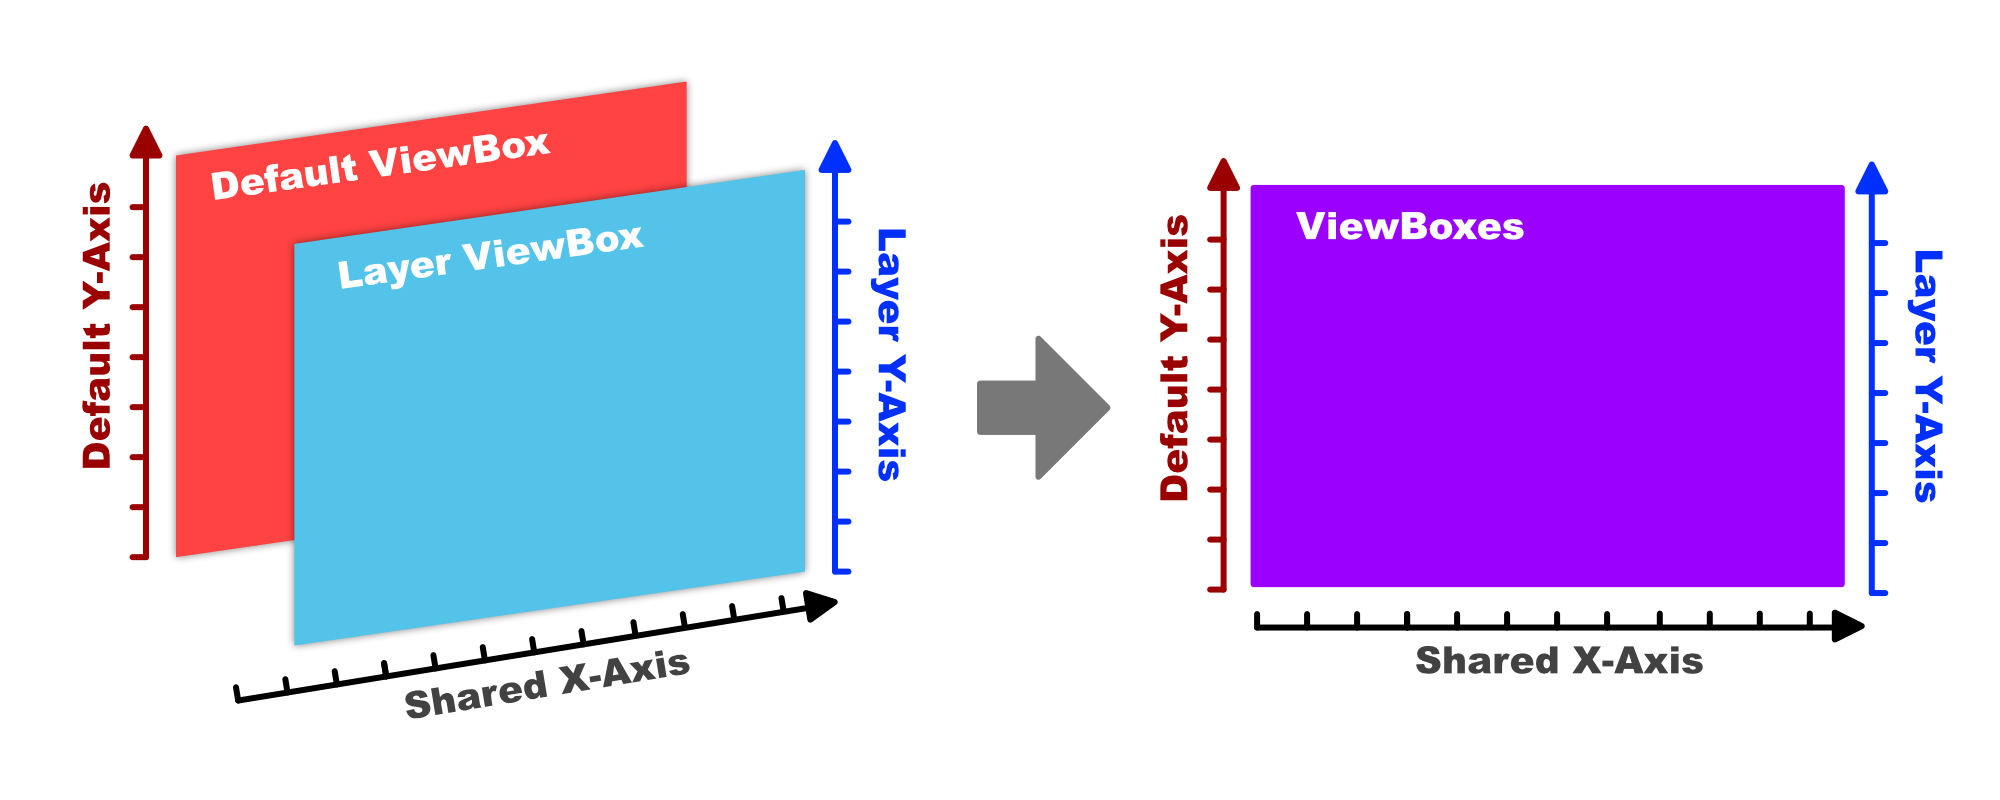
\includegraphics[width=14cm]{resources/img/PyQtGraphLayers}
    \caption{Schema displaying different layers in a single plot.}
    \label{fig:application:pyqtgraph:layers}
\end{figure}

The other addition made to PyQtGraph is a convenience layer on top of different types of data visualizations, which allow much easier connection of processes emitting data to each data visualization item. Pure PyQtGraph does not have any way of incrementally feeding data into a plot, it only allows replacing the entire data set. As an example we assume a user, who wants to display the last hour of data coming from a process, which is continously emitting new data with a frequency of 1 Hz. With pure PyQtGraph the user will have to handle saving and creating a subset of data, he is interested in all by himself. Additionally, data coming from a data loggin system, which contains data with older time stamps compared to the ones from the live data, these points will have to be sorted into the existing array of data. The reason for that is, that PyQtGraph draws the connection between points by their position in the passed array, not by the x values provided. Additionally creating a subset of the last one hour of data for an unsorted data set will be a much harder task compared to a sorted data set. The convenience layer for PyQtGraph does remove these tasks from the users responsiblities by allowing him to define a time range he is actually interested in and the only feed new data to the graph without having to store or sort it.

To achieve this, three different components have been introduced: the Update Source, the Data Model and the View. The Update Source is responsible for connecting to a device. The data model is responsible for storing the data and keeping it sorted. The View is responsible for displaying the data from the datamodel. Depiction \ref{fig:application:pyqtgraph:updatesource} shows the communication between these different layers. Operations marked in red are the intial setup of the connection between the components. Blue operatoins show the flow of data published from a process which is supposed to be visualized.

\begin{figure}[h]
    \centering
    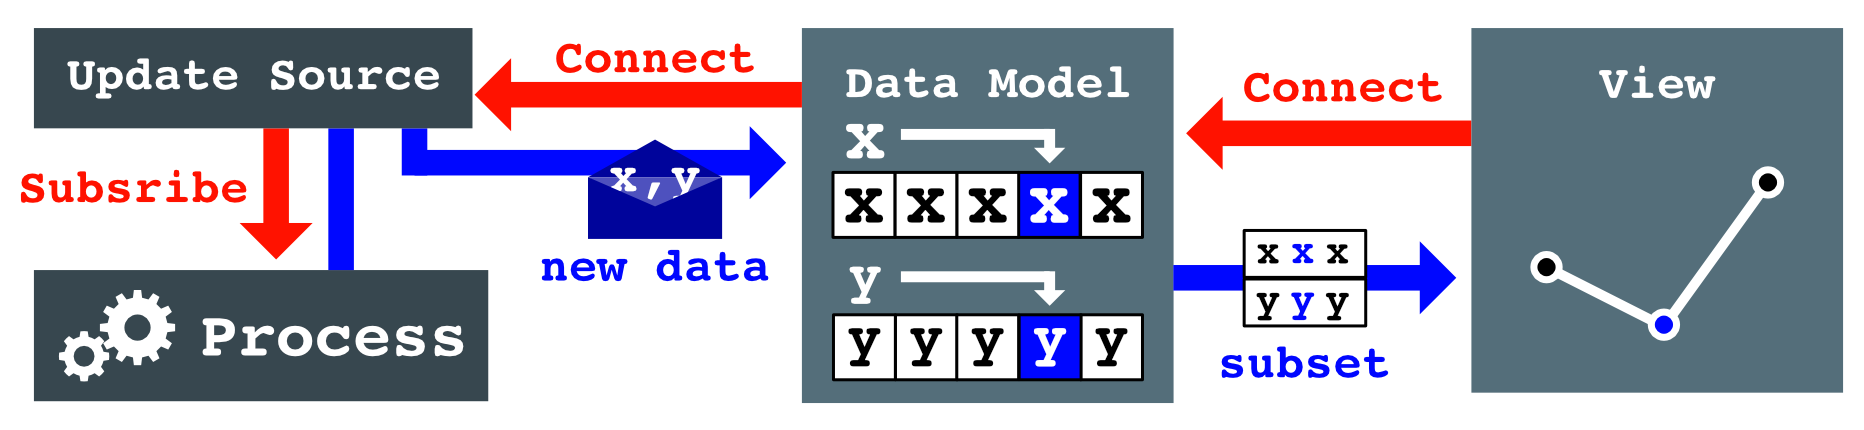
\includegraphics[width=14cm]{resources/img/PyQtGraphUpdateSource}
    \caption{Live Plotting Architecture for PyQtGraph. Operations for the initial connection are marked red, the data flow for new data is marked blue.}
    \label{fig:application:pyqtgraph:updatesource}
\end{figure}

Both, pure PyQtGraph as well as the extended versions will be included in our benchmarks, especially to investigate potential performance hits introduced by the new live data plotting architecture.



%% ==============================================
%%                   Design
%% ==============================================

\section{Design}
\label{sec:application:design}

After having a closer look at the two plotting libraries we will focus on, this chapter will focus on the design of the benchmarking framework, which we can use to investigate performance of both in the different use cases.

\subsection{Architecture}
\dots

\subsection{Benchmarking Mechanism}
\dots

\subsection{Profiling}
\dots




%% ==============================================
%%             Implementation
%% ==============================================

\section{Implementation}
\label{sec:application:implementation}

\subsection{Implementation of the Framework}
\dots

\subsection{Implementation of the Use Cases}
\dots
